\section{Experiments}\label{sec:experiments}
In this work, we take four applications including Matrix Multiplication (MM), FIR, Kmean and Sobel edge detector (Sobel) as our benchmark. To investigate the scalability of the accelerator design methodologies, each application is further provided with three different data sets ranging from Small(S), Medium(M) to Large(L) ones. The basic parameters and configurations of the benchmark are illustrated in \tabref{tab:benchmark-config} and the complete loop structure of the benchmark is presented in \tabref{tab:loop-structure}.

\begin{table}[htpb]
  \tbl{Detailed Configurations of the Benchmark \label{tab:benchmark-config}}{
  \centering
  \begin{tabular}{l|l|l|l|l}
  \hline
  Benchmark & MM & FIR & Sobel & Kmean \\ \hline
  Parameters & Matrix Size & \tabincell{l}{\# of Input \\ \# of Taps+1} & \tabincell{l}{ \# of Vertical Pixels \\ \# of Horizontal Pixels} & \tabincell{l}{\# of Nodes \\ \# of Centroids \\ Dimension Size} \\ \hline
  S & 10 & 40/50 & 8/8 & 20/4/2 \\ \hline
  M & 100 & 10000/50 & 128/128 & 5000/4/2  \\ \hline
  L & 1000 & 100000/50 & 1024/1024 & 50000/4/2 \\ \hline
  \end{tabular}
  }
\end{table}

\begin{table}[htpb]
  \tbl{Complete Loop Structure of the Benchmark \label{tab:loop-structure}}{
  \centering
  \begin{tabular}{l|l|l|l|l}
  \hline
  Benchmark & MM & FIR & Sobel & Kmean \\ \hline
  S & $10 \times 10 \times 10$ & $40 \times 50$ & $8 \times 8 \times 3 \times 3$ & $20 \times 4 \times 2$ \\ \hline
  M & $100 \times 100 \times 100$ & $10000 \times 50$ & $128 \times 128 \times 3 \times 3$ & $5000 \times 4 \times 2$  \\ \hline
  L & $1000 \times 1000 \times 1000$ & $100000 \times 50$ & $1024 \times 1024 \times 3 \times 3$ & $50000 \times 4 \times 2$ \\ \hline
  \end{tabular}
  }
\end{table}

The benchmark is implemented on Zedboard using both direct HLS based design methodology and QuickDough. Then the design productivity, implementation efficiency, performance and scalability of the two design methodologies are compared respectively.

\subsection{Experiment Setup}
All the runtimes were obtained from a laptop with Intel(R) Core(TM) i5-3230M CPU and 8GB RAM. Vivado HLS 2013.3 was used to transform the compute kernel to hardware IP Catalog i.e. IP core. Vivado 2013.3 was used to integrate the IP core and build the FPGA accelerator. The SCGRA was initially developed in ISE 14.7, and then the ISE project was imported as an IP core in XPS 14.7. With the SCGRA IP core, the SCGRA overlay based FPGA accelerator was further integrated and implemented in PlanAhead 14.7. The accelerators developed using both design methodologies targets at Zedboard \cite{zedboard} and the system works at bare-metal mode.

Direct HLS typically achieves the trade-off between hardware overhead and performance through altering the loop unrolling factors. Larger loop unrolling factors typically promise better simulation performance while more hardware resources like DSP blocks will be required and the implementation frequency may also be affected. In this work, we set the loop unrolling factor large enough to reach the best simulation performance and the detailed loop unrolling setup can be found in \tabref{tab:loop-unrolling-setup-vivado}. Larger block size is beneficial to data reuse and helps to amortize the initial communication cost, so we set the block size as large as the data buffer size. Detailed block setup of the benchmark is presented in \tabref{tab:loop-unrolling-setup-vivado} as well.

\begin{table}[htpb]
\centering
\tbl{Loop Unrolling \& Blocking Setup Of Accelerators Using Direct HLS Based Design Methodology \label{tab:loop-unrolling-setup-vivado}}{
\begin{tabular}{ll|l|l|l|l}
\hline
\multicolumn{2}{l|}{\multirow{2}{*}{Application}} & \multicolumn{2}{l|}{Max-Buffer} & \multicolumn{2}{l}{2k-Buffer} \\ \cline{3-6}
\multicolumn{2}{l|}{} & Unrolling Factor & Block Structure & Unrolling Factor & Block Structure \\ \hline

\multicolumn{1}{l|}{\multirow{3}{*}{MM}} & S & $2 \times 10 \times 10$ & $10 \times 10 \times 10$ & $2 \times 10 \times 10$ & $10 \times 10 \times 10$  \\ \cline{2-6} 
\multicolumn{1}{l|}{}                    & M & $1 \times 1 \times 100$ & $100 \times 100 \times 100$ & $1 \times 100$ & $10 \times 100$  \\ \cline{2-6} 
\multicolumn{1}{l|}{}                    & L & $1 \times 500$ & $50 \times 1000$ & 500 & 1000  \\ \hline

\multicolumn{1}{l|}{\multirow{3}{*}{FIR}} & S & $2 \times 50$ & $40 \times 50$ & $2 \times 50$ & $40 \times 50$  \\ \cline{2-6} 
\multicolumn{1}{l|}{} & M & $2 \times 50$ & $10000 \times 50$ & $2 \times 50$ & $1000 \times 50$  \\ \cline{2-6} 
\multicolumn{1}{l|}{} & L & $2 \times 50$ & $50000 \times 50$ & $2 \times 50$ & $1000 \times 50$  \\ \hline

\multicolumn{1}{l|}{\multirow{3}{*}{Sobel}} & S & $1 \times 2 \times 3 \times 3$ & $8 \times 8 \times 3 \times 3$ & $1 \times 2 \times 3 \times 3$ & $8 \times 8 \times 3 \times 3$ \\ \cline{2-6} 
\multicolumn{1}{l|}{} & M & $1 \times 1 \times 3 \times 3$ & $128 \times 128 \times 3 \times 3$ & $1 \times 1 \times 3 \times 3$ & $23 \times 128 \times 3 \times 3$ \\ \cline{2-6} 
\multicolumn{1}{l|}{} & L & $1 \times 1 \times 3 \times 3$ & $75 \times 1024 \times 3 \times 3$ & $1 \times 1 \times 3 \times 3$ & $4 \times 1024 \times 3 \times 3$ \\ \hline

\multicolumn{1}{l|}{\multirow{3}{*}{Kmean}} & S & $20 \times 4 \times 2$ & $20 \times 4 \times 2$ & $20 \times 4 \times 2$ & $20 \times 4 \times 2$  \\ \cline{2-6} 
\multicolumn{1}{l|}{} & M & $5 \times 4 \times 2$ & $5000 \times 4 \times 2$ & $5 \times 4 \times 2$ & $1000 \times 4 \times 2$  \\ \cline{2-6} 
\multicolumn{1}{l|}{} & L & $5 \times 4 \times 2$ & $25000 \times 4 \times 2$ & $5 \times 4 \times 2$ & $1000 \times 4 \times 2$  \\ \hline
\end{tabular}
}
\end{table}

QuickDough has similar design choices to those of direct HLS based design methodology in terms of loop unrolling and blocking. However, the design constrains using the two design methodologies are different. The unrolled part in QuickDough is transformed to DFG which can further be scheduled to the SCGRA overlay, so the loop unrolling factor is mainly constrained by the resources of the SCGRA overlay such as SCGRA size, instruction memory size and data memory size. As for the blocking, the design constrain in QuickDough is relatively more complex. First of all, the block size is also limited by the size of input/output buffer, which is exactly the same with the constrain using direct HLS based design methodology. In addition, the address buffer size can be another major constrain because we need to store all the IO buffer address sequence of the whole block execution instead of the DFG execution. Even though we set address buffer size twice larger than the data buffer size, it can still be a bottleneck in some occasions. The detailed SCGRA overlay configuration and corresponding loop unrolling as well as blocking setup using QuickDough are listed in \tabref{tab:scgra-config} and \tabref{tab:loop-unrolling-setup-scgra} respectively. 

\begin{table}[htpb]

\tbl{SCGRA Configuration \label{tab:scgra-config}}{
\centering
\begin{tabular}{c|c|c|c|c|c}

\hline
{SCGRA Topology} & {SCGRA Size} & {Instruction Mem} & {Data Memory} & {I/O Data Buffer} & {Addr Buffer} \\ \hline
{Torus} & {$2 \times 2$, $5 \times 5$} & {$1024 \times 72$ bits} & {$256 \times 32$ bits} & {$2048 \times 32$ bits} & {$4096 \times 18$ bits} \\ \hline
\end{tabular}
}
\end{table}


\begin{table}[htpb]
\centering
\tbl{Loop Unrolling and Blocking Setup For Accelerators Using QuickDough \label{tab:loop-unrolling-setup-scgra}}{
\begin{tabular}{l|l|l|l|l|l|l|l}
\hline
\multicolumn{2}{l|}{\multirow{2}{*}{Application}} & \multicolumn{3}{l|}{SCGRA 2x2} & \multicolumn{3}{l}{SCGRA 5x5}  \\ \cline{3-8}
\multicolumn{2}{l|}{} & \tabincell{l}{Unrolling \\ Factor} & \tabincell{l}{DFG \\ (OP/IO)} & \tabincell{l}{Block \\ Structure} & \tabincell{l}{Unrolling \\ Factor} & \tabincell{l}{DFG \\ (OP/IO)} & \tabincell{l}{Block \\ Structure} \\ \hline

\multirow{3}{*}{MM} & S & $10 \times 10 \times 10$ & 1000/301 & $10 \times 10 \times 10$ & $10 \times 10 \times 10$ & 1000/301 & $10 \times 10 \times 10$  \\ \cline{2-8} 
            & M & $5 \times 100$ & 750/606 & $10 \times 100$ & $5 \times 100$ & 750/606 & $10 \times 100$  \\ \cline{2-8} 
            & L & 200 & 301/402 & 1000 & 200 & 301/402 & 1000  \\ \hline

\multirow{3}{*}{FIR} & S & $40 \times 50$ & 860/131 & $40 \times 50$ & $40 \times 50$ & 860/131 & $40 \times 50$  \\ \cline{2-8} 
                  & M & $20 \times 50$ & 1000/141 & $100 \times 50$ & $50 \times 50$ & 2500/201 & $250 \times 50$ \\ \cline{2-8} 
                  & L & $20 \times 50$ & 1000/141 & $100 \times 50$ & $50 \times 50$ & 2500/201 & $250 \times 50$ \\ \hline

\multirow{3}{*}{Sobel} & S & $4 \times 8 \times 3 \times 3$ & 1080/39 & $8 \times 8 \times 3 \times 3$ & $8 \times 8 \times 3 \times 3$ & 2160/55 & $8 \times 8 \times 3 \times 3$   \\ \cline{2-8} 
                  & M & $4 \times 8 \times 3 \times 3$ & 1080/39 & $8 \times 8 \times 3 \times 3$ & $23 \times 8 \times 3 \times 3$ & 6210/115 & $65 \times 8 \times 3 \times 3$  \\ \cline{2-8} 
                  & L & $4 \times 4 \times 3 \times 3$ & 540/31 & $16 \times 4 \times 3 \times 3$ & $16 \times 4 \times 3 \times 3$ & 2160/55 & $16 \times 4 \times 3 \times 3$  \\ \hline

\multirow{3}{*}{Kmean} & S & $20 \times 4 \times 2$ & 920/62 & $20 \times 4 \times 2$ & $20 \times 4 \times 2$ & 920/62 & $20 \times 4 \times 2$  \\ \cline{2-8} 
                 & M & $25 \times 4 \times 2$ & 1144/72 & $125 \times 4 \times 2$ & $125 \times 4 \times 2$ & 5768/272 & $500 \times 4 \times 2$  \\ \cline{2-8} 
                 & L & $25 \times 4 \times 2$ & 1144/72 & $125 \times 4 \times 2$ & $125 \times 4 \times 2$ & 5768/272 & $500 \times 4 \times 2$   \\ \hline
\end{tabular}
}
\end{table}

\subsection{Design Productivity}
Design productivity involves many different aspects such as the abstraction level of the design entry, compilation time, design reuse, and design portability, and it is difficult to compare all the aspects, especially some of them can hardly be quantified. In this section, we mainly concentrate on the compilation time while discussing the rest briefly.

In order to implement an application on a CPU + FPGA accelerator system, direct HLS based design methodology roughly consists of the following four steps including compute kernel synthesis, kernel IP generation, accelerator implementation and software compilation.
 
\begin{itemize}
\renewcommand\labelitemi{$\bullet$}
\setlength\itemindent{1em}
\item Compute kernel synthesis: High level language program kernel is translated to an HDL model according to the user's synthesis pragma. 
\item Kernel IP generation: The compute kernel is synthesized and packed as an IP core. At the same time, the timing constrain is met and the corresponding driver is generated. 
\item Accelerator implementation: The IP core is integrated into the accelerator and the whole accelerator is implemented on the FPGA. 
\item Software compilation: The application employing the FPGA accelerator is compiled to binary code as conventional software.
\end{itemize}


Implementing an application using QuickDough also involves four steps including DFG generation, DFG scheduling, bitstream generation and software compilation.
\begin{itemize}
\renewcommand\labelitemi{$\bullet$}
\setlength\itemindent{1em}
\item DFG generation: The high level language program kernel is translated to DFG.
\item DFG scheduling: The DFG is scheduled to the customized SCGRA overlay. 
\item Bitstream generation: The scheduling result is further integrated with the pre-built accelerator bitstream to produce the new bitstream for the target application. 
\item Software compilation: Application using the SCGRA accelerator is compiled to binary code.
\end{itemize}

\figref{fig:Vivado-HLS-Compilation-Time} and \figref{fig:SCGRA-Overlay-Compilation-Time} present the compilation time of implementing the benchmark using both direct HLS based design methodology and QuickDough respectively. IP core generation and hardware implementation in direct HLS based design methodology is relatively slow. Compute kernel synthesis is usually as fast as the software compilation and can be done in a few seconds, but it may take up to 10 minutes when there is pipelined large loop unrolling involved. The last step is essentially a software compilation, and the time consumed is negligible. Basically, the direct HLS based design methodology takes 20 minutes to an hour to implement an application. With pre-implemented SCGRA overlay, the processing steps except the DFG scheduling of QuickDough are fast and the time consumed doesn't change much across different applications. DFG scheduling is relatively slower especially when the DFG size and SCGRA size are large, but it can still be completed in a few seconds. Typically, QuickDough implements an application in 5 to 15 seconds and it is already two orders of magnitude faster than direct HLS based design methodology. 

\begin{figure}[htb]
\center{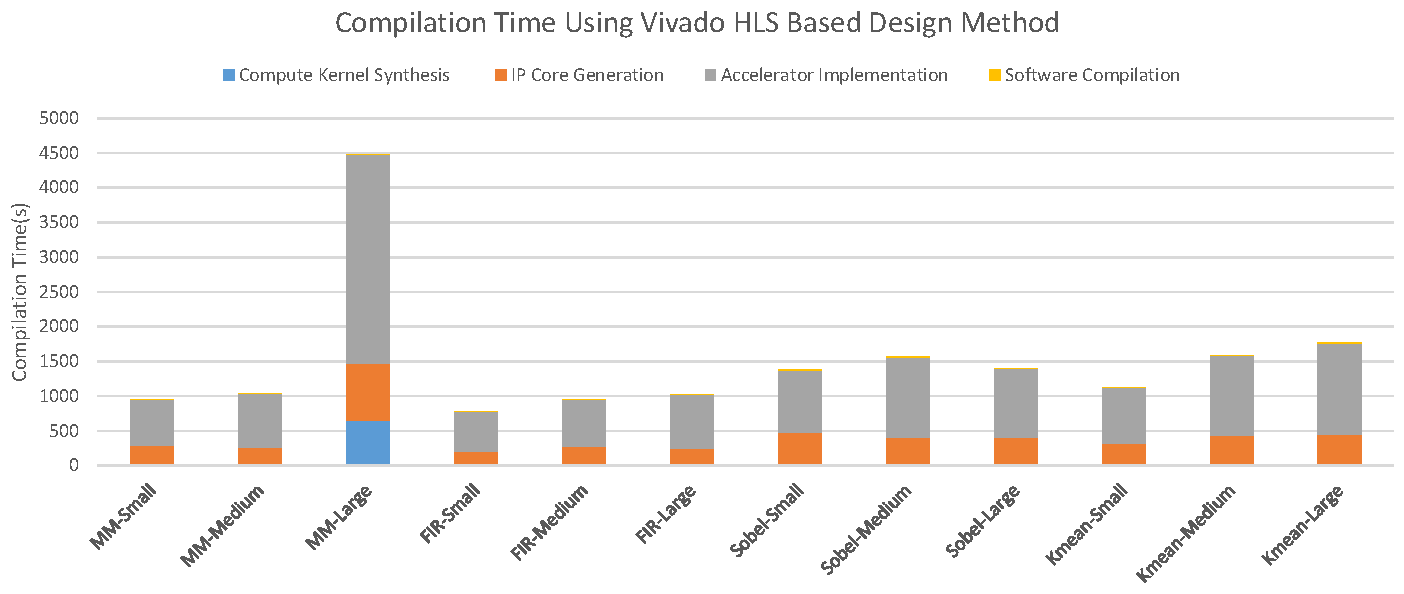
\includegraphics[width=0.8\linewidth]{HLS-Compilation-Time}}
\caption{Benchmark Compilation Time Using Direct HLS Based Design Methodology}
\label{fig:Vivado-HLS-Compilation-Time}
\end{figure}

\begin{figure}[htpb]
\center{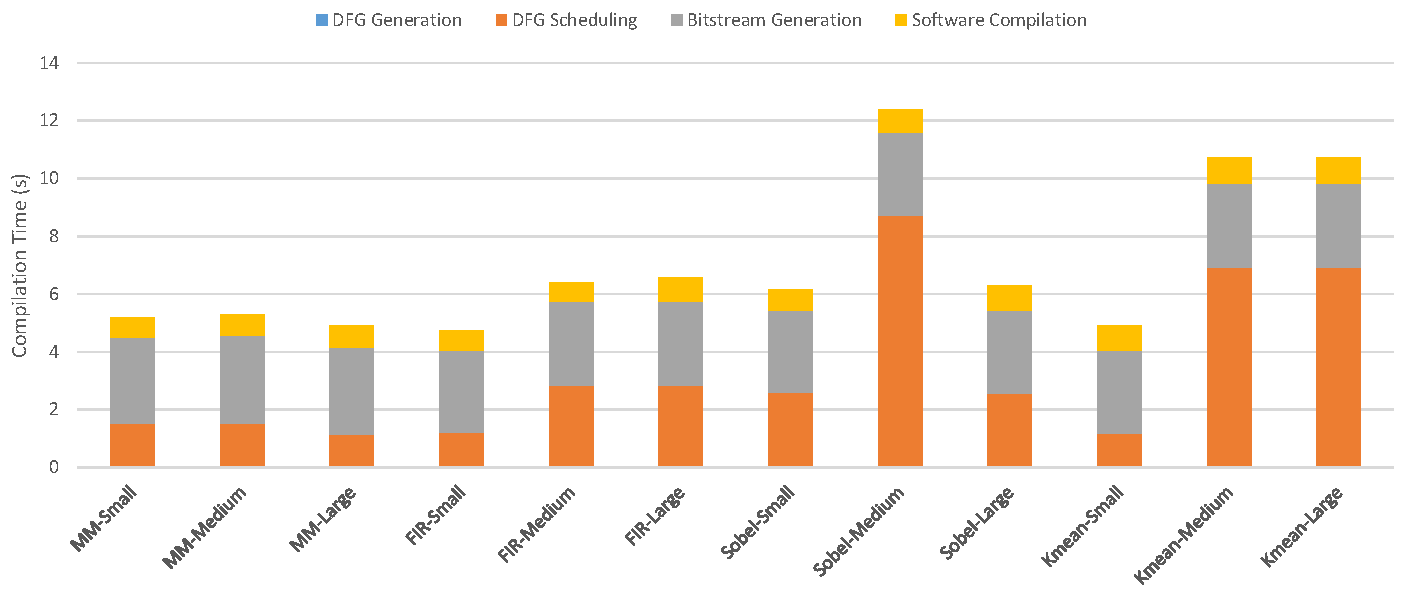
\includegraphics[width=0.8\linewidth]{QuickDough-Compilation-Time}}
\caption{Benchmark Compilation Time Using QuickDough}
\label{fig:SCGRA-Overlay-Compilation-Time}
\end{figure}

On top of the compilation time, the abstraction level of the design entry, design reuse and portability are also important aspects that affect the design productivity. Both direct HLS based design methodology and QuickDough adopt sequential high level language C/C++ as design input, but QuickDough still needs further efforts to have the DFG generation done automatically. Direct HLS based design methodology needs the compute kernel be synthesized and implemented for each application instance. QuickDough requires compilation for each application instance as well, but it can reuse the same hardware infrastructure across the applications in the same domain. It is possible for direct HLS based design methodology to port the synthesized HDL design among different devices and parts, but IP core generation and accelerator implementation depend on specific FPGA device and they are needed for each application instance. QuickDough's portability is also limited at HDL level, and complete hardware implementation is needed to port to a different FPGA device.

\subsection{Hardware Implementation Efficiency}
In this section, hardware implementation efficiency including the hardware resource overhead and implementation frequency of the accelerators using both direct HLS based design methodology and QuickDough are compared. At the same time, SCGRAs with customized operations are implemented and the hardware resource saving is analyzed.

\tabref{tab:hardware-overhead-comparison} exhibits the hardware overhead using both accelerator design methodologies. It is clear that the accelerators using direct HLS based design methodology typically consume less FF, LUT and RAM36 due to the delicate customization for each application instance. However, the number of DSP48 required increases significantly with the expansion of the application kernel and it limits the maximum loop unrolling factors for many applications. The accelerators using QuickDough usually cost comparable DSP48, more FF, LUT and particularly RAM36 which limits the maximum SCGRA that can be implemented on the target FPGA and further constrains the maximum loop unrolling and blocking as well.

\begin{table}[htpb]
\centering
\tbl{Hardware Overhead of The Accelerators Using Both Direct HLS Bsed Design Methodology and QuickDough \label{tab:hardware-overhead-comparison}}{
\begin{tabular}{l|l|l|l|l|l|l}
\hline
\multicolumn{3}{l|}{} & FF  & LUT & RAM36 & DSP48 \\ \hline 
\multirow{6}{*}{MM} & \multirow{3}{*}{ \tabincell{c}{2K \\ Buffer}} & Small & 4812 & 3390 & 4 & 84 \\ \cline{3-7} 
                    &                            & Medium & 4804 & 4703 & 4 & 12 \\ \cline{3-7} 
                    &                            & Large & 11107 & 11524 & 4 & 12 \\ \cline{2-7}
                    & \multirow{3}{*}{ \tabincell{c}{Max \\ Buffer}} & Small & 4826 & 3390 & 128 & 84 \\ \cline{3-7} 
                    &                             & Medium &  4251 & 4866 & 128 & 9 \\ \cline{3-7} 
                    &                             & Large & 11024 & 24890 & 128 & 12 \\ \hline

\multirow{6}{*}{FIR} & \multirow{3}{*}{ \tabincell{c}{2K \\ Buffer}} & Small & 3736 & 3570 & 4 & 27 \\ \cline{3-7} 
                     &                            & Medium & 3756 & 3872 & 4 & 27  \\ \cline{3-7} 
                     &                            & Large & 3756 & 3872 & 4 & 27 \\ \cline{2-7}
                     & \multirow{3}{*}{ \tabincell{c}{Max \\ Buffer}} & Small & 3742  & 3570 &  128 & 27 \\ \cline{3-7} 
                     &                             & Medium & 3782 & 4246 & 128 & 27 \\ \cline{3-7} 
                     &                             & Large & 3792 & 4426 & 128 & 27 \\ \hline

\multirow{6}{*}{Sobel} & \multirow{3}{*}{ \tabincell{c}{2K \\ Buffer}} & Small & 9556 & 6467 & 6 & 216 \\ \cline{3-7} 
                       &                            & Medium & 7483 & 5520 & 6 & 144 \\ \cline{3-7} 
                       &                            & Large & 7102 & 5501 & 6 & 144 \\ \cline{2-7}
                       & \multirow{3}{*}{ \tabincell{c}{Max \\ Buffer}} & Small & 9564 & 6467 & 130 & 216 \\ \cline{3-7} 
                       &                             & Medium & 7496 & 5711 & 130 & 144 \\ \cline{3-7} 
                       &                             & Large & 7622 & 5904 & 130 & 144 \\ \hline

\multirow{6}{*}{Kmean} & \multirow{3}{*}{ \tabincell{c}{2K \\ Buffer}} & Small & 2826 & 3567 & 4 & 24 \\ \cline{3-7} 
                       &                            & Medium & 6709 & 8088  & 4 & 120 \\ \cline{3-7} 
                       &                            & Large & 6709  & 8088  & 4  & 120 \\ \cline{2-7}
                       & \multirow{3}{*}{ \tabincell{c}{Max \\ Buffer}} & Small & 2852 & 3567 & 128 & 24 \\ \cline{3-7} 
                       &                             & Medium & 6754 & 8122 & 128 & 120 \\ \cline{3-7} 
                       &                             & Large & 6770 & 8205 & 128 & 120 \\ \hline

\multicolumn{3}{l|}{SCGRA 2x2} & 9302 & 5745 & 32 & 12  \\ \hline
\multicolumn{3}{l|}{SCGRA 5x5} & 34922 & 21436 & 137 & 75 \\ \hline
\multicolumn{3}{l|}{FPGA Resource} & 106400 & 53200 & 140 & 110 \\ \hline
\end{tabular}
}
\end{table}

To further investigate the hardware overhead, we divided the four benchmarks into three groups to implement customized SCGRAs for each of them. MM and FIR share the same operations, so they are implemented using the same SCGRA overlay. Sobel edge detector doesn't need complete 32-bit data with, and a mixed 16-bit and 32-bit data width SCGRA overlay is customized for it. Kmean which covers almost all the operations adopts the original SCGRA overlay. \figref{fig:hardware-saving} shows the hardware saving using customized SCGRA overlay. The customized SCGRA overlay can save as much as 65\% DSP48, 30\% LUT and 15\% FF.

\begin{figure}[htpb]
\center{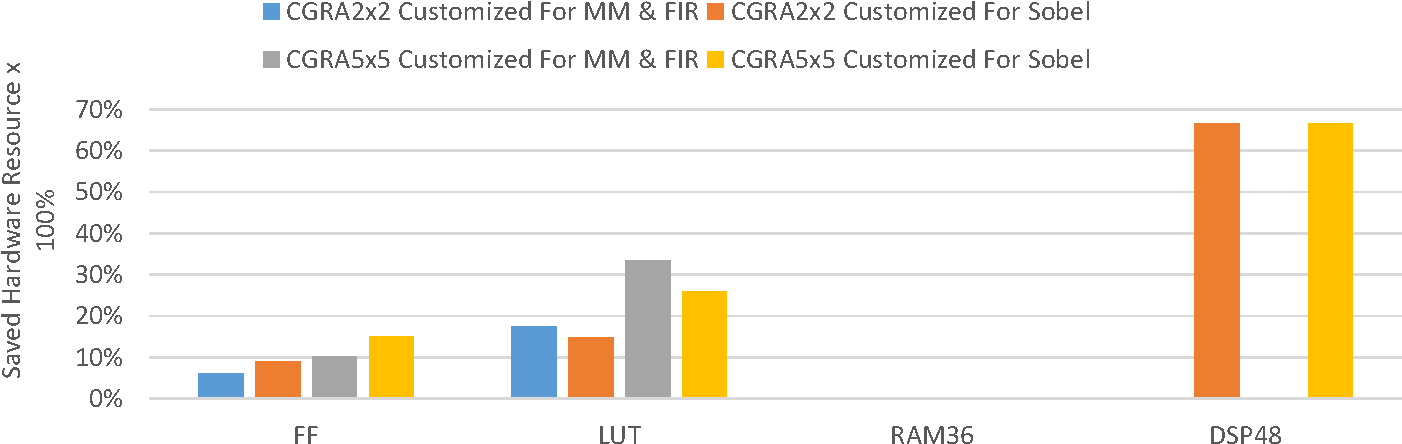
\includegraphics[width=0.8\linewidth]{hardware-saving}}
\caption{Hardware Saving Of Customized SCGRA Overlay}
\label{fig:hardware-saving}
\end{figure}

\figref{fig:impl-freq} presents the implementation frequency of the benchmark using both design methodologies. Direct HLS based design methodology takes timing constrain into consideration at the HLS step, and it can either synthesize the compute kernel to a lower frequency design with better simulation performance or a higher frequency design with worse simulation performance. Neither of them have a clear advantage over the other. The AXI controller on Zedboard typically works at 100MHz and higher frequency design requires delicate placing and routing. As a result, we set the HLS timing constrain at 100MHz and have the whole accelerator implemented synchronously. Although the current design option is not necessarily optimal, it is representative. In fact, the synthesized IP core sometimes can be even slower though we set the timing at 100MHz during HLS.

QuickDough utilizes the SCGRA overlay as the hardware infrastructure. Since the SCGRA overlay is regular and pipelined, the implementation frequency of the accelerator built on top of the SCGRA overlay is much higher than that of the accelerator produced using direct HLS. A 2x2 SCGRA based accelerator can run at 200MHz, and a 5x5 SCGRA based accelerator can work at 167MHz. The implementation frequency degrades slightly because more than 90\% of the BRAM blocks on target FPGA are used and the routing becomes extremely tight. As mentioned before, the AXI controller block on Zedboard is slower and runs at around 100MHz. To take advantage of the higher implementation frequency, simple synchronizers built with consecutive registers are inserted to divide the AXI controller and the SCGRA overlay into two clock domains.

\begin{figure}[htpb]
\center{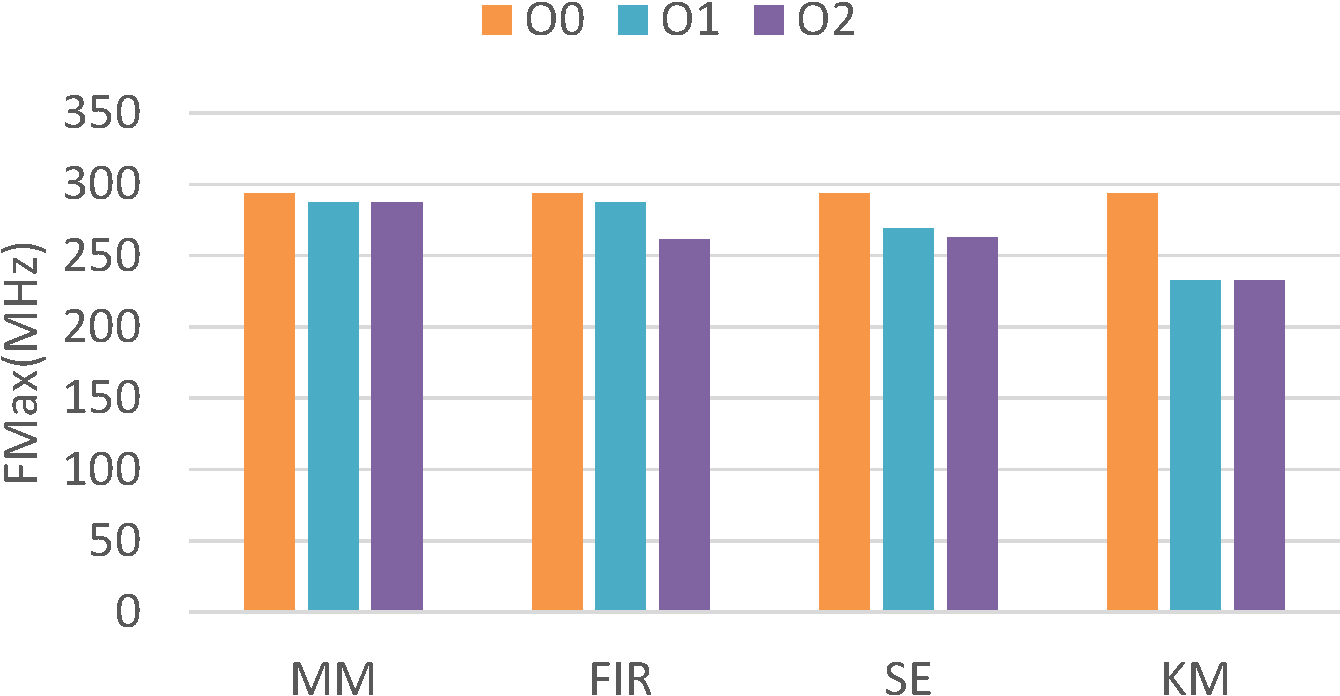
\includegraphics[width=0.8\linewidth]{impl-freq}}
\caption{Implementation Frequency of The Accelerators Using Both Direct HLS Based Design Methodology and QuickDough}
\label{fig:impl-freq}
\end{figure}

\subsection{Performance}
In this section, the execution time of the benchmark is taken as the performance metric. Since the execution time of different applications and data sets varies a lot, the performance speedup relative to direct HLS based implementation with 2k-Buffer configuration is used instead. \figref{fig:real-perf} shows the performance comparison of four different sets of accelerator implementations including two accelerators built with QuickDough and two accelerators developed with direct HLS based design methodology. According to this figure, direct HLS based design methodology presents better performance on MM-Medium, MM-Large, Sobel-Medium and Sobel-Large, while QuickDough outperforms in FIR with all three data sets, Kmean-Medium and Kmean-Large. The two design methodologies achieve similar performance on the rest of the benchmark. 

\begin{figure}[htpb]
\center{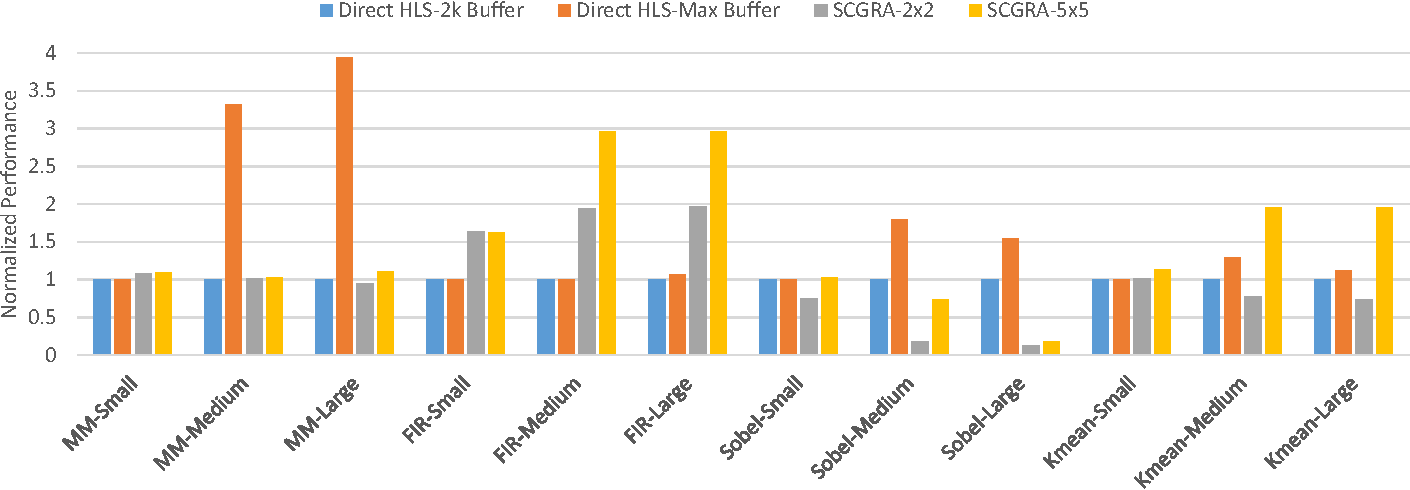
\includegraphics[width=0.8\linewidth]{real-perf}}
\caption{Benchmark Performance Using Both Direct HLS Based Design Methodology and QuickDough}
\label{fig:real-perf}
\end{figure}

To further investigate the performance of the benchmark, the distribution of the execution time including system initialization such as DMA initialization, communication between FPGA and ARM processor moving input/output data to/from the FPGA on-chip buffers, FPGA computation and the others such as input/output data reorganization for DMA transmission or corner case processing is presented in \figref{fig:execution-time}. Since the execution time of different applications with diverse data sets varies in a large range, the execution time used in this figure is actually normalized to that of a basic software implementation on ARM. 

As shown in \figref{fig:execution-time}, accelerators using direct HLS based design methodology especially the one with max-buffer configuration achieve better performance mainly through the smaller overhead in communication and 'the others' which are essentially the input/output data reorganization time. And the major reason for the lower communication and data reorganization cost is that it can accommodate larger data sets and corresponding computation for each acceleration execution, which essentially contributes to the large block size as shown in \tabref{tab:loop-unrolling-setup-vivado} because larger block size increases the data reuse between blocks and amortizes the initial DMA communication cost.

\begin{figure}[htpb]
\center{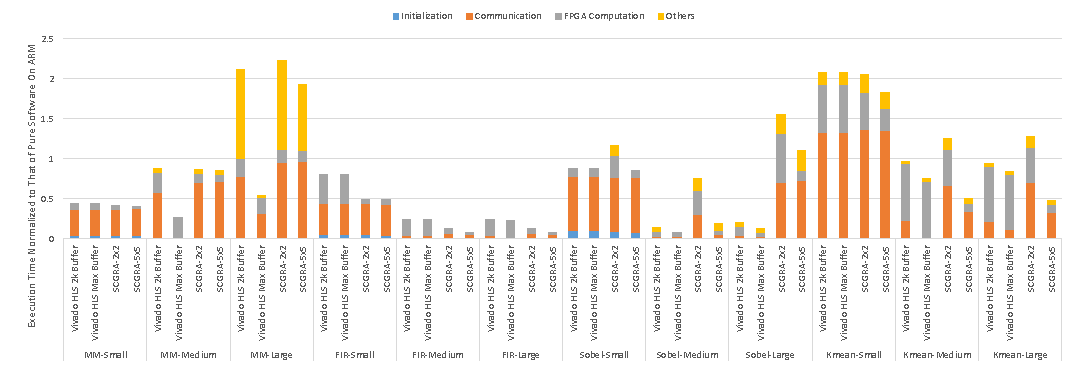
\includegraphics[width=0.99\linewidth]{execution-time}}
\caption{Benchmark Execution Time Decomposition Of The Accelerators Using Both Direct HLS Based Design Methodology and QuickDough}
\label{fig:execution-time}
\end{figure}

Computation time of QuickDough as illustrated in \figref{fig:kernel-real-perf} shows clear advantage over that of direct HLS based design methodology. As the computation time depends on both the simulation performance in cycles and implementation frequency of the hardware infrastructure, it is further analyzed from the two aspects in this section. \figref{fig:kernel-sim-perf} shows the simulation performance which is the product of the block simulation performance and the number of blocks for each compute kernel. It can be found that direct HLS based design methodology performs better on MM-Large and Sobel while QuickDough outperforms on the rest of the benchmark. Comparing the simulation performance in this figure and loop unrolling factors in \tabref{tab:loop-unrolling-setup-vivado} and \tabref{tab:loop-unrolling-setup-scgra}, we can see that the simulation performance is quite relevant to the depth of the loop unrolling. More precisely, the simulation performance mostly depends on the depth of the loop unrolling instead of the specific hardware infrastructure. The only exception in the experiments is the Sobel benchmark. And the reason is that direct HLS takes Sobel operator matrices as constant input and has the implementation optimized while the DFG generator in QuickDough just takes them as normal variables and more computations are involved. As for the hardware infrastructure, QuickDough using regular SCGRA overlay typically can run at higher frequency than the circuit generated using direct HLS and the implementation frequency contributes a lot to the advantage of QuickDough computation time. 

\begin{figure}[htpb]
\center{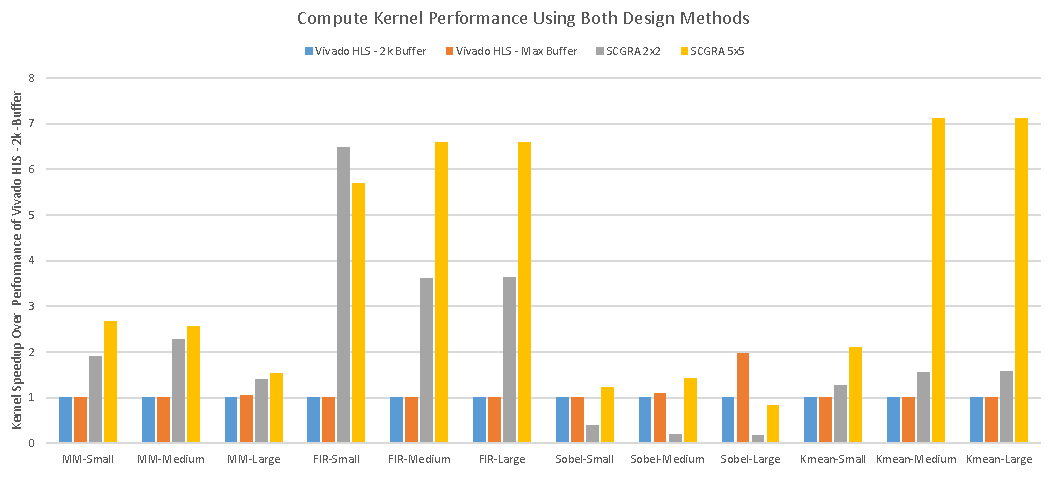
\includegraphics[width=0.8\linewidth]{kernel-real-perf}}
\caption{Compute Kernel Performance Using Both Direct HLS Based Design Methodology and QuickDough}
\label{fig:kernel-real-perf}
\end{figure}

\begin{figure}[htpb]
\center{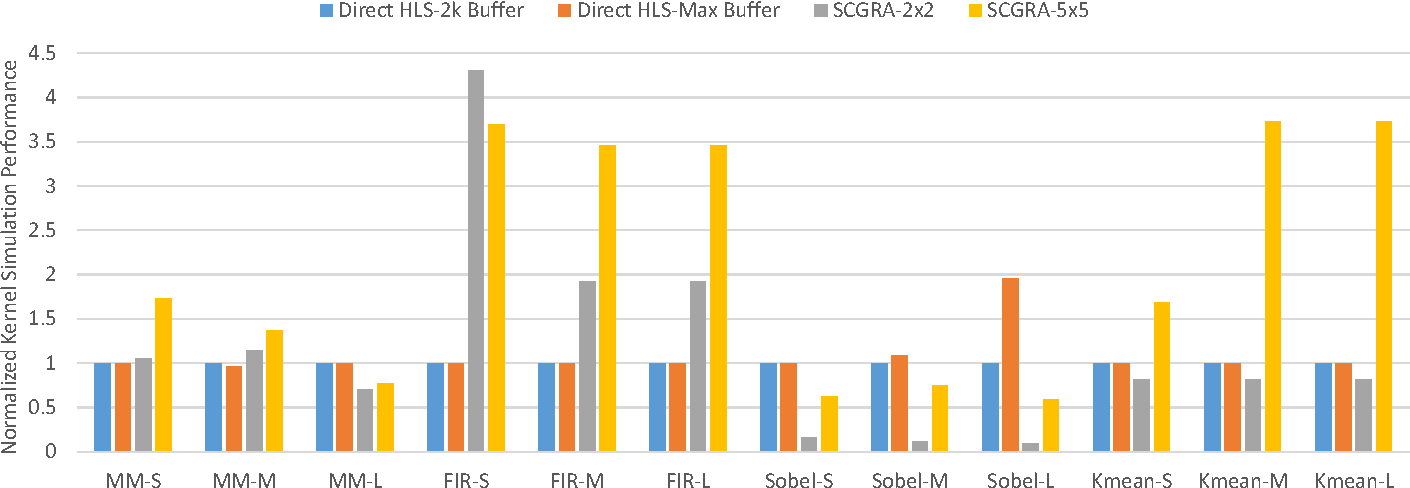
\includegraphics[width=0.8\linewidth]{kernel-sim-perf}}
\caption{Compute Kernel Simulation Performance Using Both Direct HLS Based Design Methodology and QuickDough}
\label{fig:kernel-sim-perf}
\end{figure}

In summary, the accelerators using direct HLS based design methodology can afford larger buffer and accommodate larger block size, which helps to reduce the communication time and the cost of input/output organization. Therefore, when there are more data reuse among neighboring blocks, the accelerators using direct HLS based design methodology achieves better performance. QuickDough using SCGRA overlay can provide both higher simulation performance with larger loop unrolling capability in many cases and higher implementation frequency with its regular structure, so it outperforms when the target application has smaller data set or more intensive computation.  

  
\subsection{Scalability}
On top of the design productivity, hardware implementation and performance, the scalability of the accelerator using both design methodologies is equally important. To further investigate the scalability of the two design methodologies, we use matrix multiplication with gradually increasing matrix size as a lightweight benchmark. Since FPGA resource on Zedboard is quite limited, Zc706 with abundant hardware resource is used as the target platform for scalability analysis. 

\figref{fig:mm-sim-perf} shows the simulation performance of matrix multiplication implemented using both design methodologies. Note that direct HLS with proper unrolling in this figure indicates the minimum loop unrolling that achieves the maximum performance under the hardware constrain. According to the figure, the performance of the accelerators using direct HLS based design methodology is much better than that using QuickDough when the matrix size is small enough for fully loop unrolling. When the matrix size gets larger, direct HLS can no longer afford the hardware overhead for intensive loop unrolling and the performance of the corresponding accelerator starts to degrade. In this experiment, MM-8x8 is the turning point that QuickDough begins to outperform, while the matrix size of the turning point on Zedboard is much smaller because of the limited hardware resource.

\begin{figure}[htpb]
\centering
\subfloat[]{
\label{fig:mm-sim-perf1}
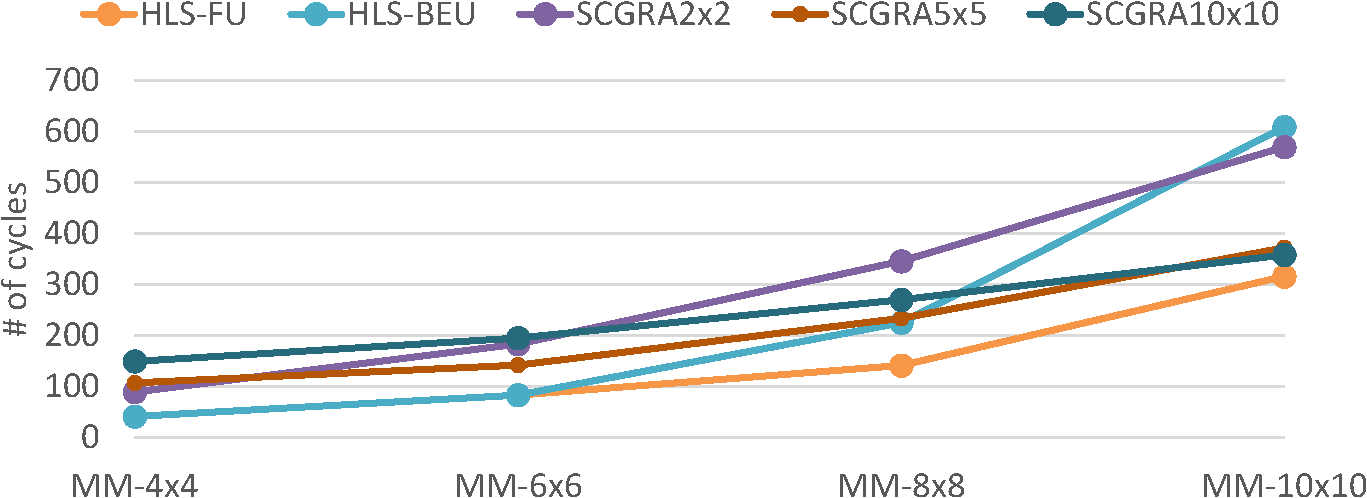
\includegraphics[width=0.4\linewidth]{mm-sim-perf1}}
\qquad
\subfloat[]{
\label{fig:mm-sim-perf2}
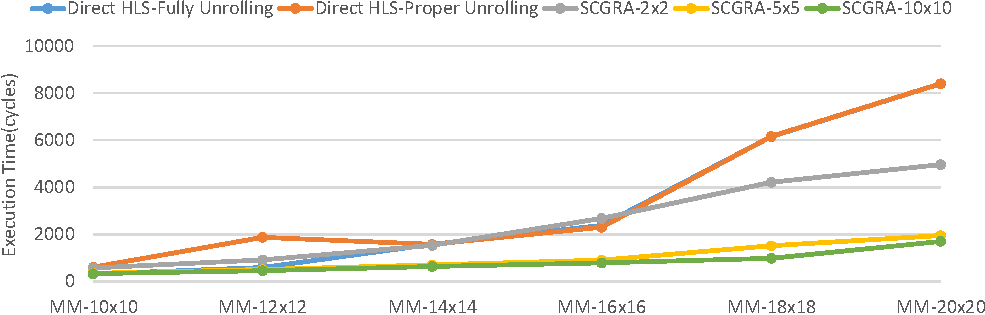
\includegraphics[width=0.48\linewidth]{mm-sim-perf2}}
\caption{Simulation Performance Of The Matrix Multiplication Using Both Direct HLS Based Design Methodology And QuickDough}
\label{fig:mm-sim-perf}
\end{figure}


When the matrix size gets to 14 as shown in \figref{fig:mm-sim-perf2}, the simulation performance using proper loop unrolling and that using fully loop unrolling starts to overlap. The major reason is that direct HLS develops both loop level parallelism through pipeline and data level parallelism through loop unrolling. When the matrix is small, direct HLS depends more on loop unrolling for performance enhancement. When the matrix is larger, loop level parallelism becomes significant to the performance and may even reach the IO bound. To further prove this statement, we have a 20x20 matrix multiplication synthesized using direct HLS with pipelining and gradually increasing loop unrolling. \figref{fig:loop-unroll-and-pipeline} shows the influence of loop unrolling and pipelining on both performance and hardware overhead. It can be found that loop unrolling typically can improve performance and requires more hardware overhead. When the loop level parallelism is big enough to consume the IO bandwidth, loop unrolling is not necessary for improving the performance. IO bandwidth instead of hardware resource turns to be the performance bottleneck. 

\begin{figure}[htpb]
\center{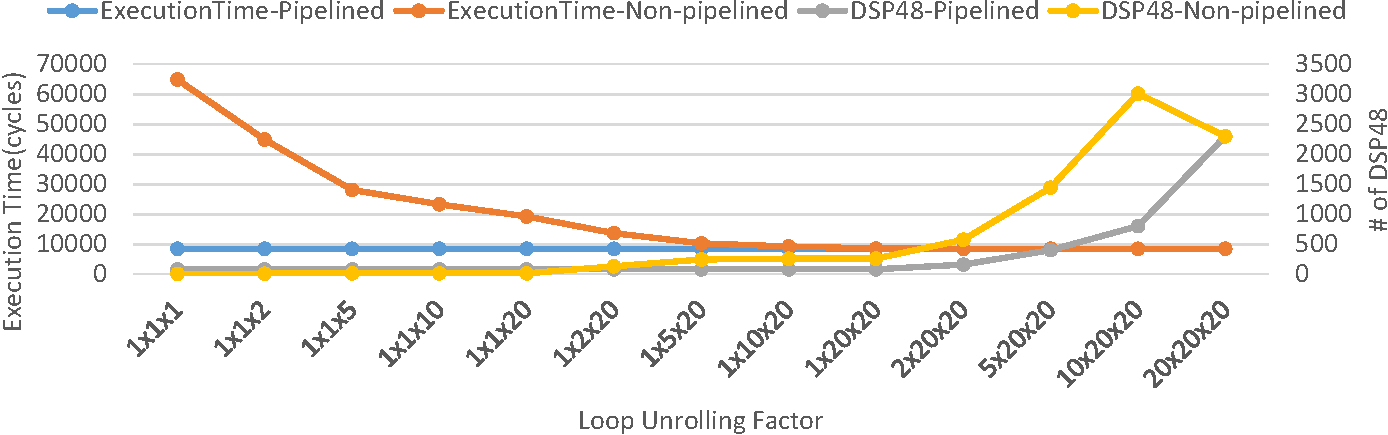
\includegraphics[width=0.8\linewidth]{loop-unroll-and-pipeline}}
\caption{MM 20x20 Implemented Using Direct HLS Based Design Methodology With Diverse Loop Unrolling And Pipelining}
\label{fig:loop-unroll-and-pipeline}
\end{figure}

However, as shown in \figref{fig:mm-sim-perf2}, when the matrix size is larger than 8x8, the accelerator using QuickDough achieves better performance than that using direct HLS with loop unrolling and pipelining. The advantages mainly lie on the following two aspects. On the one hand, SCGRA overlay can accommodate larger loop unrolling and are less prone to reach the hardware resource bottleneck, though it usually consumes larger amount of hardware resource in general. \figref{fig:scgra-overhead-scalability} shows the hardware overhead with increasing SCGRA size and it proves its scalability on hardware overhead. On the other hand, the SCGRA overlay has distributed data memory to store temporary data and allows larger loop unrolling. Thus it requires less IO bandwidth compared to the direct HLS based design and is less sensitive to the IO bound. 

\begin{figure}[htpb]
\center{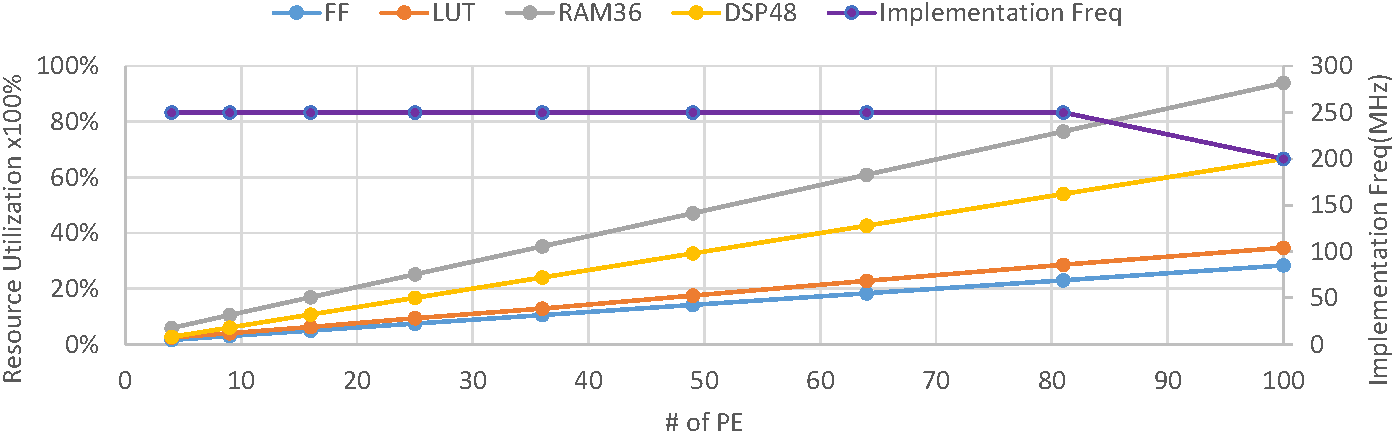
\includegraphics[width=0.8\linewidth]{scgra-impl-scalability}}
\caption{Hardware Overhead With Increasing SCGRA Size}
\label{fig:scgra-overhead-scalability}
\end{figure}

Finally, we also compare the implementation frequency using both design methodologies. Since the maximum clock available is 250MHz and the speed level of FPGA on Zc706 is -2, the implementation using both design methodologies present similar implementation frequency. QuickDough allows SCGRA ranging from 2x2 to 9x9 running at 250MHz on Zc706. SCGRA 10x10 degrades slightly and can still work at 200MHz. Direct HLS has all the implementation running at 200MHz. 
